\documentclass[tikz, border=0pt]{standalone}
\usepackage{tikz}
\usetikzlibrary{arrows,automata,positioning}

\begin{document}
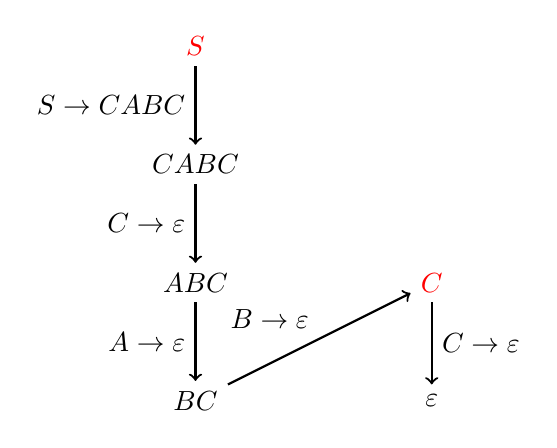
\begin{tikzpicture}[node distance=1.5cm, thick, auto]
% draw the states
\node[red] (1) {\(S\)};
\node (2) [below of=1] {\(CABC\)};
\node (3) [below of=2] {\(ABC\)};
\node (4) [below of=3] {\(BC\)};
\node[red] (5) [right of=3, xshift=1.5cm] {\(C\)};
\node (6) [below of=5] {\(\varepsilon\)};
% draw the edges
\path[->] 
(1) edge node [swap] {\(S \to CABC\)} (2)
(2) edge node [swap] {\(C \to \varepsilon\)} (3)
(3) edge node [swap] {\(A \to  \varepsilon\)} (4)
(4) edge node {\(B \to \varepsilon\)} (5)
(5) edge node {\(C \to \varepsilon\)} (6)
;
\end{tikzpicture}
\end{document}